\chapter{Ejemplo de acta de reunión}
\label{sec:ActasDeReunion}

En este Anexo se muestra cómo se desarrolla una reunión (tanto de WebMakeUp, como del PFG) o más bien el acta que se genera.

Cabe destacar que las actas quedan recogidas en la Wiki (Anexo \ref{sec:Wiki}). El siguiente acta se transforma del lenguaje WikiMedia\footnote{El lenguaje Wikimedia se utiliza para redactar documentos en una Wiki.} al lenguaje \LaTeX\footnote{\LaTeX es un lenguaje de marcas para redactar documentos formales.} gracias a Pandoc\footnote{Sitio web de Pandoc: \url{http://johnmacfarlane.net/pandoc/try/}}, que es un transformador de documentos.

A lo largo del PFG se realizan más de 30 reuniones, el poner el acta de todas era excesivo y poco provechoso, por ello se muestra este ejemplo. En todas las reuniones se deja constancia de 3 aspectos fundamentales: qué se había hecho (trabajo previamente realizado), por donde había que seguir (temas tratados) y cómo se reparten las tareas a realizar (tareas).

Este ejemplo concreto es de una reunión de WebMakeUp. Se produce en una de las primeras fases, donde se están buscando cómo interpretar y definir las interacciones. Asimismo también se tratan algunos temas relaciones con la GUI (\emph{Graphical user interface}, o interfaz de usuario).

\textbf{Fecha}

17 de Octubre de 2013

\textbf{Duración}

45' aprox.

\textbf{Asistentes}

\begin{itemize}
\itemsep1pt\parskip0pt\parsep0pt
\item
  Óscar
\item
  Haritz Medina
\item
  Cristóbal
\item
  Iñigo
\end{itemize}

\textbf{Trabajos previamente realizados}

\begin{itemize}
\item Búsqueda de información sobre SCxml\footnote{SCXml: un estandar para denotar FSMs en XML y abstracción del control de la misma. Más información: \url{http://www.w3.org/TR/scxml}}, cómo trabaja con Javascript. Modelar el funcionamiento de Wikilayer en base a un diagrama de transición de estados.
\item Pensar en cómo se podría adecuar la interfaz y mostrar un prototipo definitivo.
\item Búsqueda sobre proyectos o código fuente libre que ayuden a ahorrar tiempo en la implementación del editor.
\end{itemize}
\textbf{Temas tratados}

\begin{itemize}
\itemsep1pt\parskip0pt\parsep0pt
\item
  Definir qué 3 tipos de tareas se han de tener en cuenta:

  \begin{itemize}
  \itemsep1pt\parskip0pt\parsep0pt
  \item
    Cómo concebir una aumentación (Diseño de la aumentación).
  \item
    Cómo va a ser el IDE de desarrollo y cómo se va a implementar.
  \item
    Cómo se van a codificar extensiones (o implementar aumentaciones).
  \end{itemize}
\item
  Presentación de la herramienta Asana: planificación del trabajo del
  grupo

  \begin{itemize}
  \itemsep1pt\parskip0pt\parsep0pt
  \item
    Reparto de tareas en Asana: definir tareas, deadlines, etc.
  \item
    Designar quienes harán el seguimiento del cumplimiento de las
    tareas: Óscar y Cristóbal.
  \end{itemize}
\item
  Definir tiempo de inversión en el TFG para Haritz: 20 horas semanales
  aproximadamente.
\end{itemize}

\textbf{Tareas}

Las tareas se podrán ver con mayor precisión en la web
\href{https://app.asana.com/0/8179240639112/8179240639112}{Asana}

\underline{Tareas Haritz}

\begin{itemize}
\itemsep1pt\parskip0pt\parsep0pt
\item
  Búsqueda de librerías de Javascript que puedan ser útiles para la
  implementación de codificar o generar aumentaciones.
\item
  Trabajar con ConstraintJS, entender su funcionamiento y desarrollar un
  boceto de Wikilayer con él.
\end{itemize}

\underline{Tareas Cristóbal}

\begin{itemize}
\itemsep1pt\parskip0pt\parsep0pt
\item
  Definir un STD para wikilayer.
\item
  Definir un STD para las herramientas de Iker e Itziar y realizar pruebas de ``estrés'' de las aplicaciones con tal de buscar más requisitos para Webmakeup.
\end{itemize}

\underline{Tareas Iñigo}

\begin{itemize}
\itemsep1pt\parskip0pt\parsep0pt
\item
  Ver si es interesante la utilización de las herramientas MockingBird y Pencil o alguna de las ideas o concepciones de las mismas.
\item
  Buscar ideas que puedan ser interesantes para el IDE.
\item
  Decidir el diseño del IDE.
\end{itemize}

\underline{Tareas Óscar}

\begin{itemize}
\itemsep1pt\parskip0pt\parsep0pt
\item
  Seguimiento y control
\end{itemize}

\textbf{Próxima reunión}
Próxima semana


\chapter{Herramientas de Gestión}
\label{sec:HerramientasGestion}

En este anexo se describen las principales herramientas que se han utilizado para el PFG relacionadas con la planificación y gestión del mismo.

\section{Asana}
\label{sec:Asana}

Asana \footnote{Sitio web de Asana: \url{http://www.asana.com}} es la plataforma de planificación que se utiliza dentro del proyecto WebMakeUp entre los cuatro integrantes. Asana es un sitio web que utiliza el grupo Onekin para poder trabajar con tareas, deadlines, insertar comentarios, compartir ficheros de distintos servicios de nube (Dropbox, GoogleDrive, Box,...) en equipo. Su utilización es bien sencilla, en la Figura \ref{fig:Asana} se muestra la interfaz principal, en la cual se hace todo el trabajo. 

Asana permite tener varios proyectos en el mismo repositorio, en la imagen se muestra el proyecto WebMakeUp. En el panel marcado de color amarillo están las tareas generales actualmente en el proyecto. Estas tareas, haciendo clic en una de ellas se despliega toda la información en la parte derecha. Arriba se definen las subtareas y el deadline (resaltado de color rojo). En el centro (resaltado de azul) están los ficheros compartidos por los miembros del grupo en esta tarea. Por último, en la parte inferior (resaltado de verde) se puede realizar comentarios y hacer \emph{follow} (abonarse a que informen de los cambios en esta tarea).

Esta plataforma permite una gestión rápida y sencilla de todo el trabajo. Es sencillo para los usuarios y para que el director pueda hacer un seguimiento y control.
\begin{figure}
\begin{center}
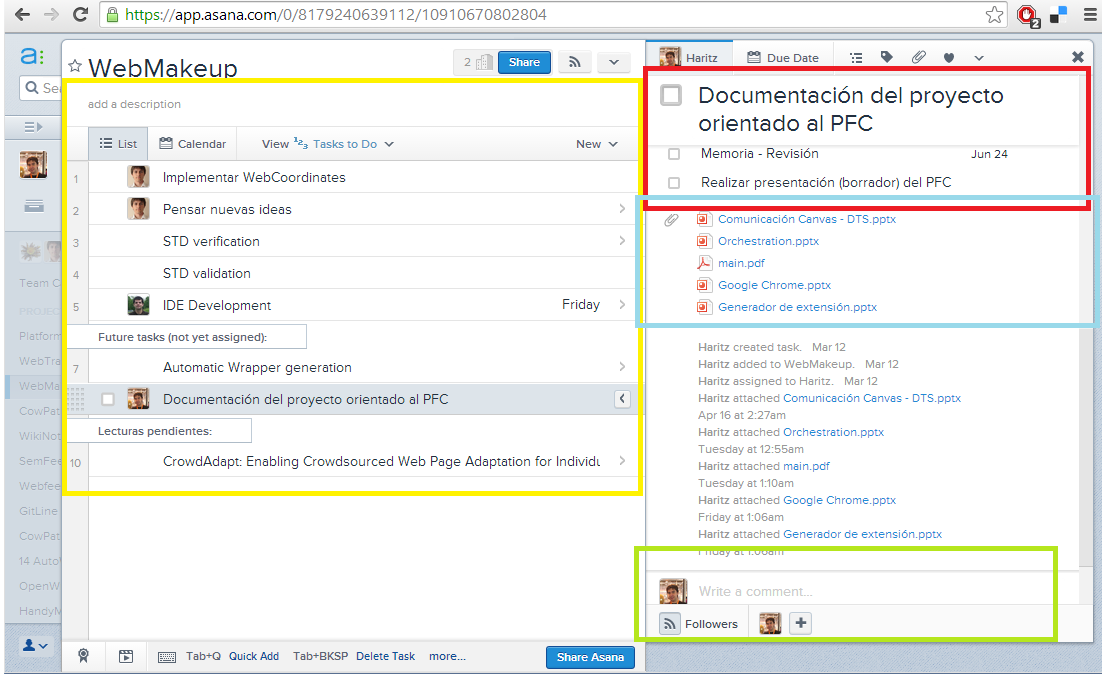
\includegraphics[width=0.95\textwidth]{figs/6-Asana.png}
\end{center}
\caption{Plataforma de TeamWork Asana}
\label{fig:Asana}
\end{figure}

\section{Wiki}
\label{sec:Wiki}

Para describir qué es una wiki, hay que poner a Wikipedia\footnote{Sitio web de Wikipedia: \url{http://en.wikipedia.org/}} como ejemplo. En Wikipedia, al igual que en cualquier wiki, hay artículos sobre diferentes cosas, donde los diferentes usuarios de ella pueden colaborar cambiando o adaptando ese contenido según dispongan de información. Esta herramienta es colaborativa y permite escribir artículos con una sintaxis bastante sencilla y además de manera concurrente entre más de un usuario.

En este PFG en concreto, Onekin ofrece su wiki orientada a los PFG que dispone con tal de que se puedan ir documentando ciertos aspectos del mismo, herramientas, librerías, actas de reuniones, DOP, etc.

\section{Gestión de tareas en Access}
\label{sec:Access}

El control exhaustivo que se lleva a lo largo del proyecto, permitiendo mejorar los procesos, las estimaciones y garantizando el alcance de los objetivos, requiere de una herramienta. Para ir haciendo planificaciones, obtener estadísticas y realizar un seguimiento y control adecuado se necesita de un sistema gestión de tareas más potente que lo que se utiliza en clase. Para ello existen muchas herramientas predefinidas con tal cometido, pero tras hacer un pequeño estudio de las mismas, se decide hacer una herramienta a medida, que no solo es útil en este proyecto, si no que lo puede ser en muchos más que se planteen en el futuro. Esta herramienta desarrollada de manera personal tiene que cubrir las siguientes necesidades:
\begin{itemize}
\item{No requerir mucho tiempo de desarrollo.}
\item{Interfaz sencilla y usable.}
\item{Obtención de estadísticas de manera que se reflejara el avance de las tareas y el grado de cumplimiento.}
\end{itemize}

Al principio se comienza a realizar este control en Microsoft Excel, dado que ofrece una manera sencilla de representar. El coste de desarrollo es mínimo, se ven claro todos los datos y se pueden obtener gráficas y estadísticas de manera sencilla. Pero a medida que avanzaba el proyecto, se detectan ciertos problemas: falta de escalabilidad, falta de relación de datos (si una tarea se hace en diferentes días o no) y además se ve que no hay manera de representar tareas aplazadas a otras fechas. Esto último es importante para resolver una de las métricas de control de calidad implantadas (Apartado \ref{sec:Calidad}).

Por estas razones, se decide exportar esta gestión a Microsoft Access y su uso mediante formularios, con los que ya se ha trabajado previamente. En la Figura \ref{fig:AccessPlanificacionGestion}, se muestra cómo se dispone de un sencillo formulario para computar todas las planificaciones, seguimiento y aplazamientos de las tareas. Se definen algunas vistas (o consultas en Access), por ejemplo, para ver qué tareas están sin finalizar u obtener estadísticas de todo tipo. Gracias a ello se puede ir viendo de manera más clara si se van alcanzando los objetivos.

\begin{figure}
\begin{center}
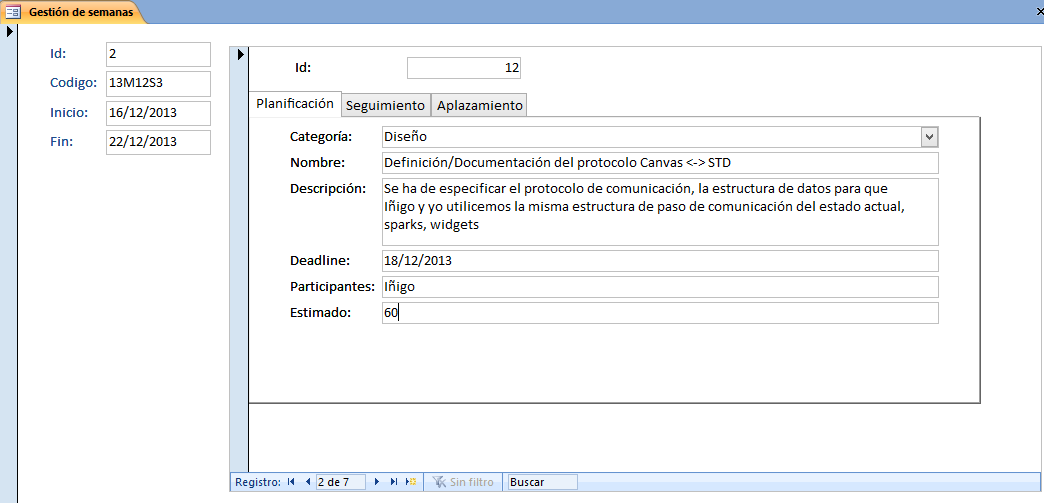
\includegraphics[width=0.95\textwidth]{figs/6-AccessPlanificacion.png}
(a)Planificación de las tareas, dividido por semanas.
\label{fig:AccessPlanificacion}
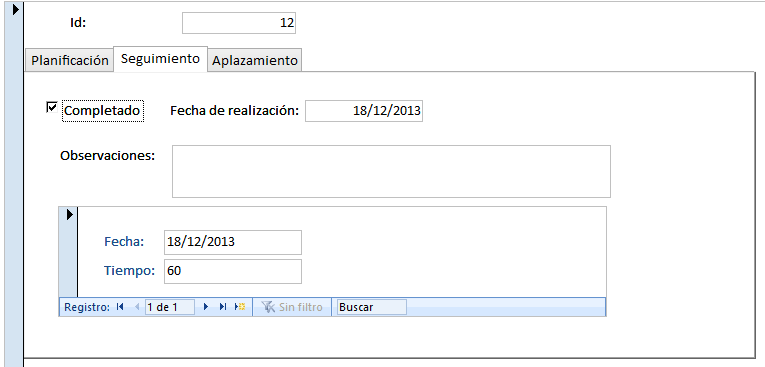
\includegraphics[width=0.95\textwidth]{figs/6-AccessSeguimiento.png}
(b)Seguimiento y control
\label{fig:AccessSeguimiento}

\caption{Sistema de gestión de tareas en Access desarrollado para el control de las tareas.}
\label{fig:AccessPlanificacionGestion}
\end{center}
\end{figure}

\section{\LaTeX{}}
\label{sec:Latex}

Tal y como lo describen en la página oficial de \LaTeX{} \footnote{Sitio web del proyecto \LaTeX{}: http://www.latex-project.org/} es un estándar \emph{de facto} para comunicar y publicar documentos de índole científica.

Las razones de utilizar \LaTeX en lugar de otras herramientas que se utilizan a lo largo de los cursos académicos (como Open/LibreOffice o Microsoft Office) son las siguientes:

\begin{itemize}
\item{Es un proyecto enorme y describirlo es complejo. Para ello modularizar la documentación es una buena práctica y con \LaTeX se puede hacer dividiéndolo en diferentes ficheros.}
\item{Hay que centrarse en las cosas a contar y no en el diseño o presentación del mismo, y en ese aspecto esta herramienta separa muy bien estos dos aspectos.}
\item{En los artículos de investigación como estándar se utiliza \LaTeX y aprender el cómo utilizarlo es importante por si se requieren usos del mismo en el futuro.}
\item{Al ser texto plano que posteriormente se procesa, permite una fácil integración con herramientas de control de versiones. En este caso se ha utilizado GIT con un repositorio en GoogleCode. El utilizar un sistema de control de versiones no es posible a día de hoy con casi cualquier otro tipo de procesador de textos.}
\item{No dependencia de servicios en nube. Por ejemplo, Google Drive cumplía con prácticamente el resto de requisitos, pero la dependencia de su servicio para poder documentar podía suponer algún riesgo, por ejemplo si el servicio dejaba de estar disponible.}
\end{itemize}

Para el aprendizaje de LaTeX y cómo referencia se ha tomado el libro \cite{WikiLatex}.

\section{GIT}
\label{sec:GIT}

GIT es un sistema de control de versiones distribuido. Se puede tanto trabajar en local cómo utilizar un repositorio, por ejemplo en la nube, con la que compartir con otra gente y poder trabajar de manera conjunta. En este caso, se realizan dos tipos de desarrollo donde GIT tiene cabida.

Por un lado el desarrollo de WebMakeUp utilizando BitBucket como servidor en nube, y por otro lado la documentación de la memoria, utilizando Google Code como servidor en nube.

Durante el proceso de planificación se ve que era necesario para el desarrollo de software en equipo la necesidad de usar un control de versiones. Con él, se resuelven muchos de los problemas que habitualmente se tienen: unión de versiones de trabajo por parte de los diferentes integrantes, log de cambios, respaldos de seguridad, etc.

Por tanto dado que apenas se trabaja en estos aspectos a lo largo del Grado en Ingeniería Informática, es necesario innovar y aprender a utilizar esta herramienta.

\section{Google Code}
\label{sec:GoogleCode}
Google Code ofrece almacenamiento en nube de proyectos software. Permite compartirlos y disponer no solo de un repositorio GIT, Mercurial\footnote{Explicación del control de versiones Mercurial: \url{http://en.wikipedia.org/wiki/Mercurial}} o Subversion\footnote{Explicación del control de versiones Apache Subversion: \url{http://en.wikipedia.org/wiki/Apache_Subversion}}, si no que además ofrece una Wiki y tramitación de incidencias. La principal ventaja frente a BitBucket es que el panel de administración es más sencillo. Al usarse para documentación donde solo hay un integrante es más conveniente utilizar esta plataforma. Google Code solo permite repositorios públicos.

En este caso la documentación y el código fuente de este documento está a disposición de cualquier usuario\footnote{Dirección del repositorio de google code con el código fuente de la memoria: \url{https://code.google.com/p/memoria-pfc/}} permitiendo nutrirse del mismo. La documentación del proyecto está pública bajo licencia GNU GPLv2\footnote{Licencia GNU GPLv2: \url{http://www.gnu.org/licenses/old-licenses/gpl-2.0.html}}.

\section{BitBucket}
\label{sec:BitBucket}
BitBucket, al igual que Google Code admite los mismos tipos de repositorio. La principal diferencia es que este permite repositorios privados, es decir, que no sean públicos y que sólo los invitados puedan tener acceso al mismo. Esto es parte de los requisitos del propio WebMakeUp y por eso se utiliza este servicio.


\section{Dropbox}
\label{sec:Dropbox}
Dropbox es una plataforma de almacenamiento en nube. En este proyecto se utiliza esta herramienta como \emph{backup} de todo el sistema de información. Las principales razones de su uso son: su fiabilidad y robustez, y un cliente que permite sincronizar diferentes ordenadores/móviles. Gracias al cliente todos los ficheros están actualizados en todos los dispositivos. Con ello, no sólo ofrecen backup en nube, si no en otros ordenadores que lo tengan sincronizado, no obligando en ningún momento a depender de la plataforma en caso de caída.


\section{GoJS}
\label{sec:Gestion-GoJS}

GoJS se utiliza en la representación de los STD de WebMakeUp con un modelo de interacciones basado en diagramas de transición de estados explicados en el Apartado \ref{sec:modeloSTD} y más concretamente en el Apartado \ref{sec:Interacciones-GoJS}. Pero GoJS es mucho más potente y se utiliza para dibujar algunos diagramas presentes en la memoria.
Estos son el diagrama de GANTT (Figura \ref{fig:Gantt}) y el organigrama de miembros de WebMakeUp (Figura \ref{fig:OrganigramaEquipo}), que están hechos con esta librería de Javascript. 

Por tanto, esta librería ha sido utilizada a lo largo del propio proyecto para describir los diagramas de transición de estados en WebMakeUp y también para poder generar parte de esta documentación. Con ello se valida aún más que el uso de ciertos elementos en WebMakeUp también pueden ser completamente válidos en otros muchos ámbitos no relacionados únicamente con desarrollo, en este caso en poder generar parte de la documentación.


\chapter{Breve manual de WebMakeUp}
\label{sec:ManualWebMakeUp}

WebMakeUp es una herramienta de aumentación web \emph{Do-it Yourself} realizada por el grupo Onekin\footnote{Sitio web del grupo Onekin: \url{http://onekin.org/}}. Varios de los aspectos del editor se elaboran en este PFG, pero para comprender en su totalidad la herramienta es recomendable describir brevemente sus características.

WebMakeUp es un editor que funciona como extensión de Google Chrome. Tras instalarla sale en el navegador en la parte derecha un nuevo icono tal y como se observa en la Figura \ref{fig:MenuWebMakeUp}.

\begin{figure}
\centering
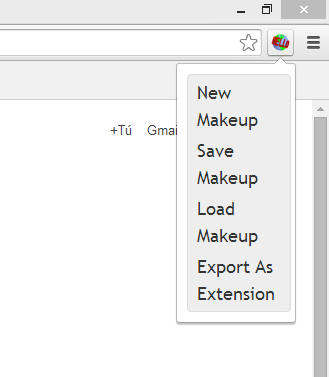
\includegraphics[width=0.45\linewidth]{./figs/A-MenuWebMakeUp}
\caption{Menú principal de WebMakeUp}
\label{fig:MenuWebMakeUp}
\end{figure}

En este menú se dispone de 4 opciones.
\begin{itemize}
\item{\textbf{New MakeUp}: permite abrir el editor y crear una nueva aumentación en la página sobre la que se está trabajando.}
\item{\textbf{Save MakeUp}: permite salvar en cualquier momento la aumentación que se está desarrollando. La aumentación queda guardada dentro del propio navegador.}
\item{\textbf{Load MakeUp}: permite cargar una aumentación previamente salvada.}
\item{\textbf{Export As Extension}: permite exportar la aumentación como extensión de Chrome. Es el paso que se realiza en este PFG en el Capítulo \ref{cha:generador}.}
\end{itemize}

Al navegar en un sitio web se puede (sin necesidad de abrir el editor) obtener clons de widgets.

Para obtener los clons pulsando el boton derecho hay una opción llamada MineIt (ver Figura \ref{fig:MenuMineIt}). Se remarcan los widgets de color a medida que se pasa el cursor por encima de ellos. Volviendo a hacer clic, se almacena ese clon en el \emph{Piggy Bank}, que es un repositorio local de widgets.

Existen actualmente dos tipos de clons, clons simples y clons complejos. Los simples son copias del contenido que se selecciona. Estos puede que se actualicen cada cierto tiempo si el motor observa que el contenido es variable (por ejemplo si es un mapa del tiempo). 

Los complejos están compuestos de dos fases. En una primera fase se tiene que recoger qué es lo que se quiere clonar. Suponiendo el ejemplo del gráfico con la puntuación de películas de \url{www.filmaffinity.com} que se observa en la Figura \ref{fig:MenuMineIt}.

\begin{figure}
\centering
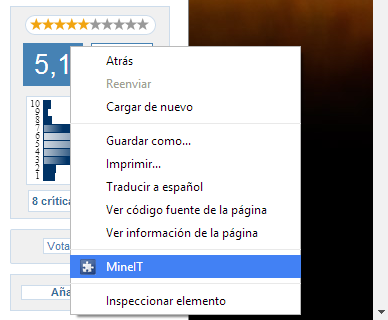
\includegraphics[width=0.45\linewidth]{./figs/A-MenuMineIt}
\caption{Menú MineIt para clonar widgets de sitios web en WebMakeUp}
\label{fig:MenuMineIt}
\end{figure}

Una vez se abre el editor WebMakeUp (pulsando en New MakeUp al navegar en un sitio web concreto), se muestran dos menús laterales (ver Figura \ref{fig:EditorWebMakeUpOpened}). El izquierdo es el \emph{Piggy Bank} y el derecho el de los patrones de diseño basados en blinks (Apartado \ref{sec:modeloBlinks}).

\begin{figure}
\centering
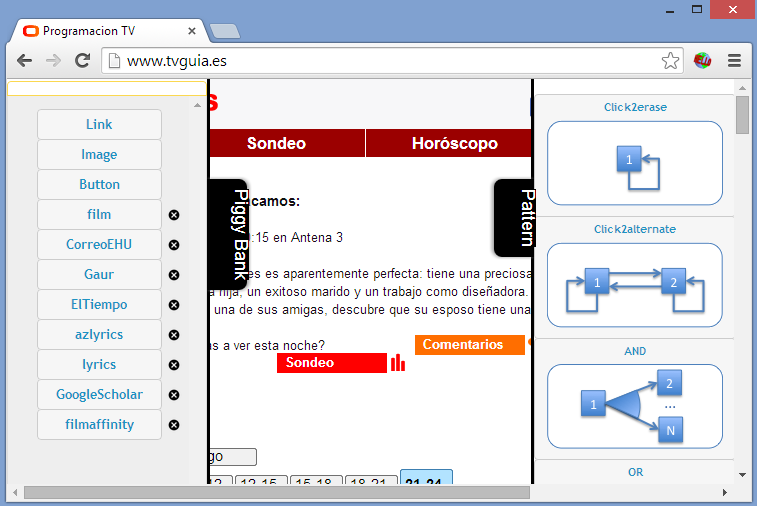
\includegraphics[width=0.55\linewidth]{./figs/A-EditorWebMakeUpOpened}
\caption{Editor WebMakeUp sobre TVGuia.es con los 2 menús laterales.}
\label{fig:EditorWebMakeUpOpened}
\end{figure}

Sobre el sitio web se remarcan los widgets de color verde a medida que se pasa el cursor por encima de ellos. Al hacer clic se convierte lo seleccionado en widget.

Desde el \emph{Piggy Bank} se pueden arrastrar y soltar también los widgets clonados de otros sitios webs que haya en el repositorio.

Una vez dispuestos los widgets sobre el Canvas, la zona de trabajo, que es el sitio web, se puede crear animaciones entre ellos. Se pueden realizar blinks arrastrando links entre widgets o bien seleccionándolos y pulsando en el panel derecho sobre el patrón que se desee. Si se opta por la segunda opción de manera automática se generan todos los links.

\begin{figure}
\centering
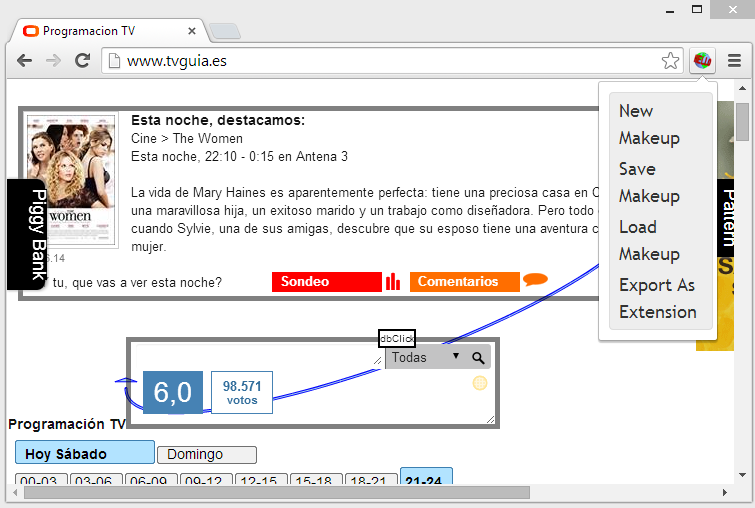
\includegraphics[width=0.55\linewidth]{./figs/A-EditorWebMakeUpAugmented}
\caption{Editor WebMakeUp sobre TvGuia con la aumentación editada}
\label{fig:EditorWebMakeUpAugmented}
\end{figure}

Finalmente, una vez se tiene la aumentación finalizada (ver Figura \ref{fig:EditorWebMakeUpAugmented}), se pulsa en \emph{Export As Extension}. Esto genera un comprimido .zip que se puede instalar como extensión en Google Chrome.

Existe más información al respecto en el artículo \cite{WISEWebMakeUp}, donde se explican los aspectos técnicos más avanzados del editor WebMakeUp y las ideas que lo avalan.

\chapter{ConstraintJS}
\label{sec:CJS}

ConstraintJS (a partir de ahora CJS) es una librería desarrollada por Stephen Oney\footnote{Sitio web de Stephen Oney: \url{http://from.so/}} que tiene como propósito principal definir restricciones en javascript de manera sencilla.

En este PFG se ha utilizado a raíz de encontrar un par de artículos sobre S.Oney \cite{Oney:2012:CPI:2380116.2380146} y 
\cite{InterState}.

El primero de ellos es un \emph{paper} sobre CJS, donde se explican las principales características de la herramienta. El segundo de ellos es sobre Interstate, que es una herramienta basada en CJS. Su objetivo es proporcionar un editor donde la interacción entre figuras geométricas se hace mediante transiciones en máquinas de estado finitas, una por cada figura geométrica.

CJS ofrece múltiples características, pero en este apartado se habla de dos. La primera, que se utiliza para comunicar el Canvas y el STD (Apartado \ref{sec:modeloSTD}) en la primera versión de WebMakeUp. La segunda, es la que se utiliza en el intérprete de las interacciones descrito en el Apartado \ref{sec:EjecucionExtension}.

CJS dispone de una API\footnote{API de CJS: \url{http://cjs.from.so/api/}} muy sencilla de usar, con unos métodos muy bien documentados y sencillos de utilizar. De igual manera, al estar todavía en fase de desarrollo de manera muy activa y con código fuente libre, se puede contactar con el autor para proponerle mejoras, cambios o correcciones.

La primera característica es que CJS permite crear \textbf{restricciones}. En CJS se definen variables y se asocia una relación con otras variables. Explicado de otra manera, definiendo que y = x + 5; si x cambia de valor, automáticamente y también cambia de valor manteniendo esa relación con x.

\begin{verbatim}
var x = cjs(3);
var y = cjs(function (){return x.get() + 5};
y.get(); //Devuelve 8
x.set(7);
y.get(); //Devuelve 12
\end{verbatim}

Esto por si sólo no es excesivamente útil, pero CJS también puede definir qué función realizar cuando se cambia una de las restricciones:

\begin{verbatim}
x.onChange(function() {
    console.log(y.get());
});
\end{verbatim}

Esto mostrará en la consola el valor de \emph{y} cada vez que cambie de valor \emph{x}.

Mediante esta técnica, la primera versión de WebMakeUp con dos áreas de trabajo (el STD y el Canvas), permite la comunicación de las mismas. Cada vez que cambia algo del STD se modifica el modelo de datos que está encapsulado en restricciones de CJS. Por tanto, cada vez que cambie algo en el modelo de datos, esto se manejará en el lado del Canvas, y viceversa.

La segunda característica de la que dispone CJS, es la de crear \textbf{máquinas de transición de estados} (a partir de ahora FSM). La FSM presenta una interfaz sencilla para generar estados, crear transiciones en base a eventos sobre elementos del DOM y manejar automáticamente las funciones a realizar cuando haya transiciones o se cambie a un estado concreto.

En el Apartado \ref{sec:EjecucionExtension} se puede observar las funciones que se han utilizado en WebMakeUp para la realización de las animaciones. Las máquinas de estado, aunque CJS las ofrece con una API sencilla, hay que tener en cuenta que internamente también están desarrolladas sobre restricciones. Con ello, se pueden definir restricciones sobre FSMs o transiciones en base a cambios en alguna de las restricciones.




























% line in order to check if utf-8 is properly configured: áéíóúñ

